\subsection{Adding a New Aspect to Your Project}
Create a new Class and name it \code{World}. Edit the buffer so it looks like listing \ref{lst:aspect} and then save it:
\begin{lstlisting}[basicstyle=\small\it,caption=An \caesarj -cclass including an aspect,label=lst:aspect,name=listing:aspect,frame=none]{}
package myPackage;

public deployed cclass World {
	
	pointcut p(HelloWorld c) : execution(void HelloWorld.sayHelloTest(String)) && this(c);
   
	after(HelloWorld d) : p(d)
	{
		System.out.println("After Hello World");
	} 
} 
\end{lstlisting}

Furthermore you will need a "'Main-Class"' to run the project. Just create one like this:

\begin{lstlisting}[basicstyle=\small\it,caption=An \caesarj -java-class including an main method,label=lst:main,name=listing:main,frame=none]{}
package myPackage;

public class MAIN {
	public static void main(String[] args) {
		HelloWorld test = new HelloWorld();
		test.sayHelloTest("Hello World");
	}
}
\end{lstlisting}

Make a clean Build of the project, and the outline view populates like in figure \ref{fig:aspect2}. Expand the \code{after()} node.

\begin{figure*}[htbp]
	\centering
		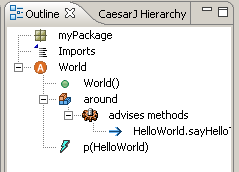
\includegraphics[width=0.35\textwidth]{images/aspect2.png}
	\caption{Outline view with content}
	\label{fig:aspect2}
\end{figure*}

You can see that this advice is affecting the \code{HelloWorld.sayHello()} method. Clicking on the \code{HelloWorld.sayHello()} node in the outline takes you to the declaration of \code{HelloWorld.sayHello()}.\\
Notice the \textit{advice annotation} in the editor buffer (highlighted) and that the \code{sayHello} method in the outline view shows that it is advised by the \textit{World aspect}. It should look like in figure \ref{fig:aspect3}.

\begin{figure*}[htbp]
	\centering
		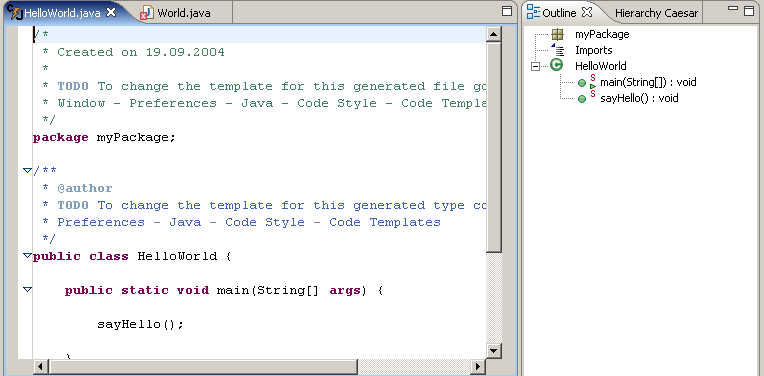
\includegraphics[width=1.0\textwidth]{images/aspect3.png}
	\caption{Advice relationship}
	\label{fig:aspect3}
\end{figure*}

Selecting the \code{World.after()} node in the outline view takes you back to the advice declaration. Right-clicking on the advice annotation brings up a context menu that also allows you to navigate to the advice.

